\chapter{Requirements and technology selection}

\FloatBarrier

\section{Assignment and acceptance approach}

The assignment is to implement the inventory workflow of Chapter 1 as an inspectable single-store application. A requirement counts as complete only when its actor, server operation, data effect and acceptance evidence can all be identified. For the approval workflows added in the expanded release, the behavior on replay, on a stale snapshot and across state changes must also be defined. A screen that appears to offer an operation is insufficient if the matching server permission or transactional behavior is missing, and a correct API is equally insufficient if the interface presents an absolute count as a relative change.


The requirements in Table~\ref{tab:requirements} are grouped into identity, catalog, stock operations, inventory inspection, warning review, reporting and administration. Correctness concerns cut across these groups: retry handling belongs to stock operations but depends on the request key kept by the browser, and cache fallback belongs to warning retrieval but depends on the database remaining the durable owner. The table therefore also serves as a map across the implementation layers.


\begingroup\small\setstretch{1.05}\setlength{\tabcolsep}{3pt}\renewcommand{\arraystretch}{1.25}
\begin{longtable}{>{\raggedright\arraybackslash}p{0.3\textwidth}>{\raggedright\arraybackslash}p{0.3\textwidth}>{\raggedright\arraybackslash}p{0.3\textwidth}}
\caption{Functional requirements and acceptance evidence}\label{tab:requirements}\\
\toprule
\textbf{ID} & \textbf{Required behavior} & \textbf{Principal acceptance evidence} \\
\midrule\endfirsthead
\toprule
\textbf{ID} & \textbf{Required behavior} & \textbf{Principal acceptance evidence} \\
\midrule\endhead
\bottomrule\endfoot
\leavevmode{}R1 & \leavevmode{}Sign in and sign out with current role authority & \leavevmode{}Anonymous denial, invalid credentials, session and role checks \\
\leavevmode{}R2 & \leavevmode{}Maintain catalog categories and suppliers & \leavevmode{}Uniqueness validation, referenced-record conflicts and archival \\
\leavevmode{}R3 & \leavevmode{}Receive and dispatch stock with an audit record & \leavevmode{}Before–delta–after arithmetic and attributed history \\
\leavevmode{}R4 & \leavevmode{}Apply signed adjustments and absolute counts & \leavevmode{}Negative correction, count-to-zero and unchanged-count cases \\
\leavevmode{}R5 & \leavevmode{}Search, filter and paginate inventory & \leavevmode{}Empty result, stable ordering and page-size boundary \\
\leavevmode{}R6 & \leavevmode{}Maintain shortage and recovery episodes & \leavevmode{}Zero, equality, severity change, recovery and expiry scenarios \\
\leavevmode{}R7 & \leavevmode{}Record managerial acknowledgement independently & \leavevmode{}Reviewer visibility and unchanged stock quantity \\
\leavevmode{}R8 & \leavevmode{}Present stock reports and selected-page export & \leavevmode{}Server aggregates, rendered reports and export scope \\
\leavevmode{}R9 & \leavevmode{}Manage users, roles and store preferences & \leavevmode{}Administrator boundary, next-request access and last-admin guard \\
\leavevmode{}R10 & \leavevmode{}Resist duplicate and concurrent stock submission & \leavevmode{}Exact replay, changed-payload conflict and concurrent tests \\
\leavevmode{}R11 & \leavevmode{}Preserve warning results without Redis & \leavevmode{}Cache bypass comparison and recorded outage equivalence \\
\leavevmode{}R12 & \leavevmode{}Track batch balances and apply FEFO/\allowbreak{}FIFO allocation & \leavevmode{}Receipt replay, expiry boundaries and batch dispatch tests \\
\leavevmode{}R13 & \leavevmode{}Detect expiry and slow-moving conditions & \leavevmode{}Business-timezone and sales-only warning tests \\
\leavevmode{}R14 & \leavevmode{}Manage replenishment and purchase approval & \leavevmode{}Suggestion quantities, approval recheck, partial receipt and cancellation tests \\
\leavevmode{}R15 & \leavevmode{}Review counts and disposal with a snapshot & \leavevmode{}Stale snapshot, approval and idempotent review tests \\
\end{longtable}\endgroup

\FloatBarrier

\section{Functional requirements}

\subsection{Authentication and role-specific access}

Users must authenticate before they can read inventory, and the server exposes the current account and role through a session-based API. Administrators manage accounts, catalog records and preferences; managers review stock health, read reports and update thresholds; clerks record movements and inspect inventory history. These are fixed role bundles rather than a configurable permission hierarchy, following the separation of roles and permissions described in the RBAC literature \citep{sandhu1996}.


Figure~\ref{fig:permissions} shows the three bundles; the administrator holds every manager and clerk permission and adds product identity, staff accounts, store settings and direct corrections. Every protected operation must be authorized by the server: navigation guards spare users misleading paths, but a caller who bypasses the browser must receive the same decision. An account disabled after sign-in must not remain usable merely because its cookie still exists, and role changes must take effect on the next request.


\begin{figure}[htbp]\centering
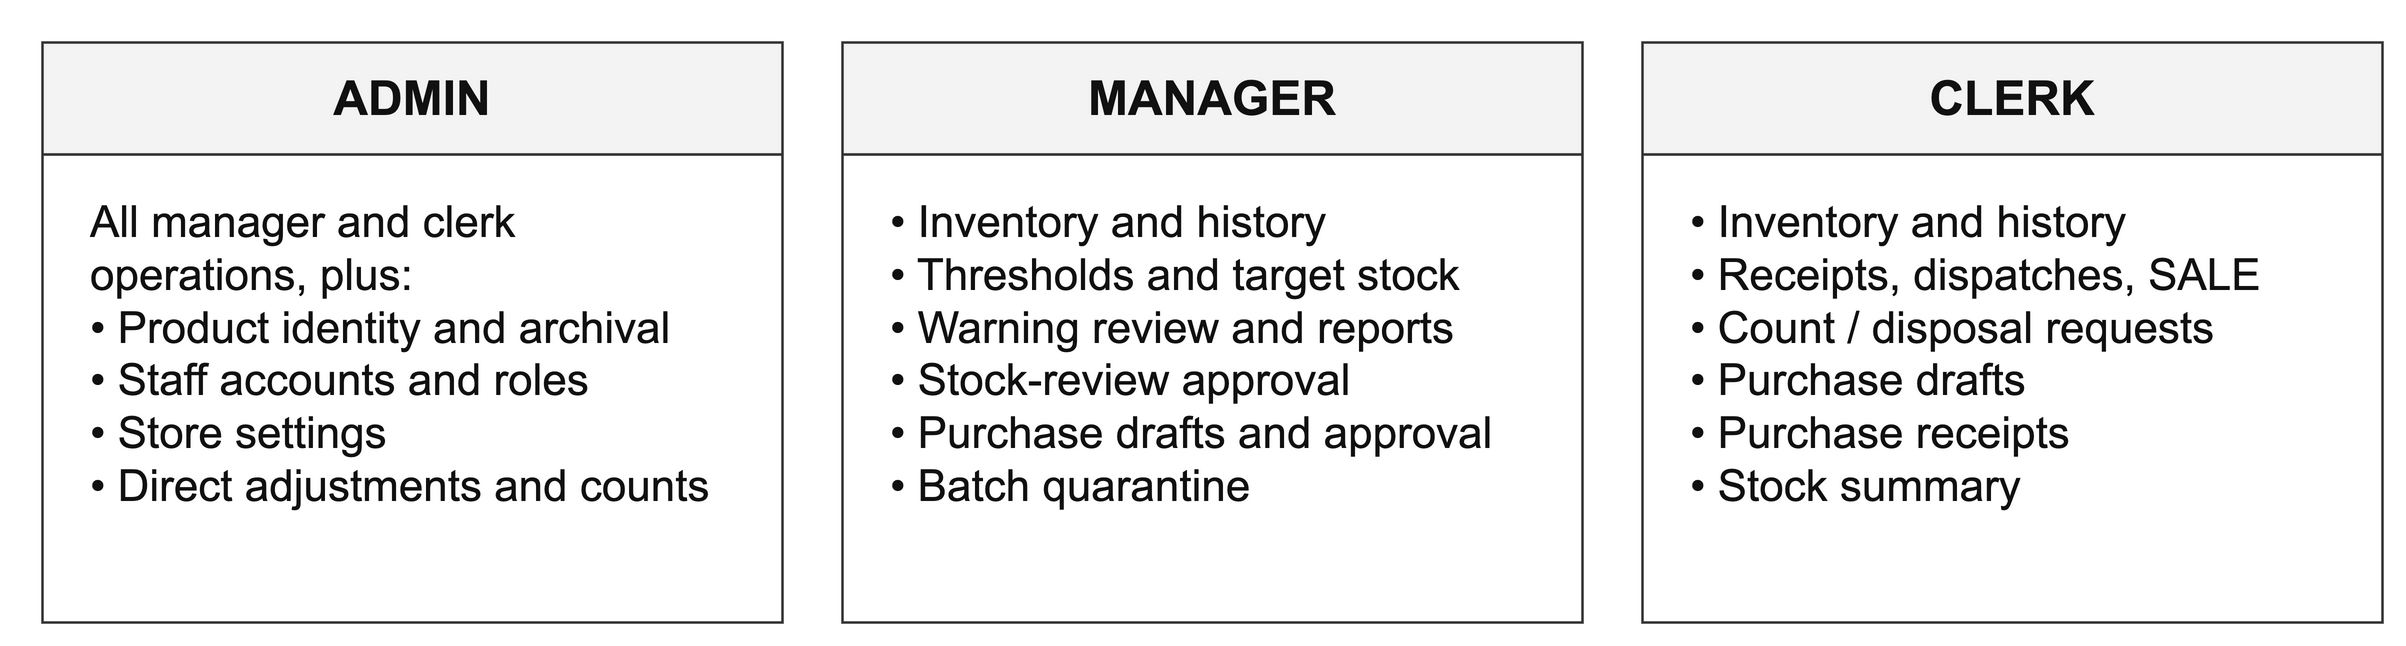
\includegraphics[width=\textwidth,height=0.70\textheight,keepaspectratio]{../figure-assets/diagrams/07-permission-model.png}
\caption{Fixed role bundles enforced by the server and reflected in navigation}\label{fig:permissions}
\end{figure}

\subsection{Catalog and inventory inspection}

Catalog administration requires unique SKUs, bounded non-negative prices, valid references and a consistent threshold hierarchy. Editing a product must not change its quantity, and archiving it must preserve its ledger while rejecting new movements. Category and supplier administration must protect existing references instead of silently detaching products on deletion.


Inventory inspection requires search by name, SKU and barcode, category selection, stock-health filters, stable sorting and bounded page sizes. The result count and pagination must describe the filtered selection, and an empty selection must offer a way to reset the filters.


For API consumers, pages are numbered from zero and their size is capped at one hundred; the interface loads twelve products per page. Sort fields are allow-listed and always end with an ID tie-breaker, which avoids ambiguous ordering and prevents a request parameter from becoming an arbitrary database expression. Snapshot consistency across pages is not promised while concurrent writes change the data.


\subsection{Stock operation requirements}

Each stock request must name a product, movement type, quantity, reason and idempotency key, while the actor is taken from the authenticated principal. The server must derive the signed effect and read the before balance under the product lock. A failed request must leave no accepted movement and no partial quantity change. An unchanged stocktake must still be recorded, because the observation itself carries information.


An exact replay must return the original transaction identifier without applying a second change, and reusing a key with different normalized content must produce a conflict. Requests that would make the quantity negative or exceed the supported maximum must be rejected. Concurrent dispatches must be serialized per product so that the successful ones can never oversell the locked balance.


\subsection{Warning and reporting requirements}

A sellable balance of zero must be classified as OUT, even when the threshold is also zero, and a positive balance equal to the reorder threshold must be LOW. Batch expiry reduces sellable quantity at the configured business-day boundary while the physical quantity remains available for disposal. A healthy replenishment must resolve the shortage and open a recovery episode. Slow-moving detection considers sales only, over a configured window. Continued low stock at the same severity must keep its reviewer, and any change to the threshold or warning policy must re-evaluate the affected episodes.


Reports must describe the recorded stock state rather than invent business indicators: inventory value uses current prices, the activity trend counts movements by UTC date, and the category mix uses current quantity totals. Acknowledgement must record who reviewed an episode without changing stock, and this distinction must be visible in labels, API operations and database relationships alike.


\FloatBarrier

\section{Non-functional requirements and quality boundaries}

Correctness takes priority over optional acceleration. MySQL must retain products, movements, warnings and settings, and neither posting stock nor retrieving authoritative warning results may depend on Redis. The movement path must update the balance, audit record, warning state and cache revision in one transaction, so that a failure rolls back the whole change instead of exposing a partial result.


The application must be reproducible from explicit dependencies and migrations. Local services are versioned in the repository, and evaluation scripts record machine, workload and sample metadata where available. Because another host may yield different latencies, reproducibility here means that the workload and procedure can be inspected and repeated, not that every recorded number will recur exactly.


Responsiveness is checked in a phone-sized viewport, with table scrolling confined to its container. The interface pairs stock colors with text labels and gives form fields descriptive names. These choices address relevant accessibility concerns, but full WCAG conformance is not claimed, since that would require a broader manual and automated assessment \citep{wcag}. Table~\ref{tab:quality} lists each quality attribute with the limits of its current evidence.


\begin{table}[htbp]\centering\small\setstretch{1.05}\setlength{\tabcolsep}{3pt}\renewcommand{\arraystretch}{1.25}
\caption{Quality requirements and limits of the current evidence}\label{tab:quality}
\begin{tabular}{>{\raggedright\arraybackslash}p{0.3\textwidth}>{\raggedright\arraybackslash}p{0.3\textwidth}>{\raggedright\arraybackslash}p{0.3\textwidth}}
\toprule
\textbf{Attribute} & \textbf{Required behavior} & \textbf{Current verification boundary} \\
\midrule
\leavevmode{}Consistency & \leavevmode{}Atomic bounded stock changes & \leavevmode{}Selected real-database transaction and concurrency cases \\
\leavevmode{}Retry handling & \leavevmode{}One accepted result per actor key and intention & \leavevmode{}Exact and conflicting replay plus same-product concurrency \\
\leavevmode{}Authorization & \leavevmode{}Server permission for each protected operation & \leavevmode{}Integration checks and browser guard scenarios \\
\leavevmode{}Recoverability & \leavevmode{}MySQL state remains authoritative without cache & \leavevmode{}Recorded Redis interruption and application restart \\
\leavevmode{}Usability & \leavevmode{}Clear stock semantics and recoverable empty states & \leavevmode{}Interface inspection and responsive browser checks \\
\leavevmode{}Performance & \leavevmode{}Described latency under a documented workload & \leavevmode{}Small sequential local warning-query benchmark \\
\leavevmode{}Maintainability & \leavevmode{}Explicit layers, schema and reproducible dependencies & \leavevmode{}Source structure, migrations and runnable scripts \\
\bottomrule\end{tabular}\end{table}

\FloatBarrier

\section{Analysis of related inventory systems}

\subsection{Reordering rules in Odoo}

Odoo's replenishment workflow uses minimum and maximum stock quantities to decide when, and how much, to reorder \citep{odoo}. Shelfwise similarly derives a replenishment suggestion from an explicit stock boundary, but the suggestion only seeds a draft purchase: submission, approval and receipt remain separate audited actions. Approval rechecks the current suggestion, and partial receipts create batch-aware movements. Supplier settlement and lead-time optimization are outside the implemented workflow.


\subsection{Retained ledger explanations in ERPNext}

ERPNext follows an immutable-ledger approach in which cancelling a document preserves the original entries and records reversing ones instead of deleting the earlier posting \citep{erpnext}. The underlying principle—accepted operational history must remain explainable after a correction—also guides Shelfwise, and ERPNext's stock ledger shows how such postings can be inspected within a larger enterprise system \citep{erpnext-stock}.


Shelfwise likewise keeps accepted movement rows and records corrections as later adjustments or stocktakes. Its audit history is, however, enforced only through the application's endpoints; a privileged database administrator can still alter stored rows directly. Document cancellation, backdated reposting and accounting integration, which ERPNext also provides, are outside Shelfwise's scope.


\subsection{Spreadsheet and broader enterprise alternatives}

A spreadsheet can serve a very small stock list well when a single person controls editing: it is easy to inspect and requires almost no deployment. The difficulty addressed here arises once several staff roles need coordinated writes, attributed changes and server-enforced permissions, which a shared worksheet could provide only with additional controls. This comparison is analytical rather than an experimental evaluation of a particular spreadsheet product.


Enterprise resource planning systems integrate inventory with purchasing, warehouse locations, finance and sales. Shelfwise instead concentrates on one store's inventory transactions, warning rules and reviewed stock workflows. The narrower scope reduces integration effort and leaves checkout, accounting and multi-store operation to later development. Table~\ref{tab:alternatives} summarizes the comparison.


\begin{table}[htbp]\centering\small\setstretch{1.05}\setlength{\tabcolsep}{3pt}\renewcommand{\arraystretch}{1.25}
\caption{Comparison of inventory-management approaches within the project scope}\label{tab:alternatives}
\begin{tabular}{>{\raggedright\arraybackslash}p{0.3\textwidth}>{\raggedright\arraybackslash}p{0.3\textwidth}>{\raggedright\arraybackslash}p{0.3\textwidth}}
\toprule
\textbf{Approach} & \textbf{Useful characteristics} & \textbf{Gap relative to this assignment} \\
\midrule
\leavevmode{}Shared stock worksheet & \leavevmode{}Simple deployment and direct visibility & \leavevmode{}Requires added controls for concurrency, roles and attributed changes \\
\leavevmode{}Documented Odoo replenishment & \leavevmode{}Quantity policies connected to replenishment & \leavevmode{}Broader enterprise and supplier scope \\
\leavevmode{}Documented ERPNext ledger & \leavevmode{}Retained posting and correction explanations & \leavevmode{}Broader document, accounting and reposting mechanisms \\
\leavevmode{}Shelfwise bounded application & \leavevmode{}Batch-aware stock, warning rules, review and purchase approval with tests & \leavevmode{}No checkout integration, accounting, multi-store isolation or store-user study \\
\bottomrule\end{tabular}\end{table}

\FloatBarrier

\section{Technology selection and comparative analysis}

\subsection{Backend and persistence}

Java 21 and Spring Boot 3.5.16 provide typed request records, validation, servlet security, JPA repositories, transaction management and health endpoints, within the Java and build-tool versions documented by the framework \citep{springboot}. The inventory-specific validation and consistency rules are implemented in the service layer.


MySQL serves as the durable relational store. Its locking reads provide a primitive for coordinating updates to a product row, and its constraints protect identities and foreign keys \citep{mysql-locks}. PostgreSQL could support an equivalent design; the choice reflects the existing project baseline and tested environment rather than a comparative benchmark. Flyway migrations define the schema, and JPA validates the mapping at startup.


Redis caches warning-page responses and nothing else. It follows the cache-aside pattern, in which a miss triggers an authoritative query and a best-effort cache fill \citep{redis-cache}. To prevent stale pages after a write, the project adds a revision namespace stored in the database. This adds a read to every query and a shared update to every relevant write, so the cache must be evaluated with these costs included rather than assumed to be faster.


\subsection{Frontend and communication}

Vue 3 provides a component-based browser interface, and TypeScript describes the response shapes used by pages and the API client \citep{vue}. Vue Router handles navigation, Pinia holds the authenticated account, Axios performs HTTP requests, Element Plus supplies the controls and ECharts renders the summaries. Responsive styles adapt the same application to desktop and phone-sized screens.


Shelfwise exposes a resource-oriented JSON API with server-side session authentication. Since Fielding lists stateless interaction among the REST constraints \citep{fielding2000}, the session-based API departs from REST in that the server retains request context. A second application node would therefore require shared sessions or session affinity.


\subsection{Development and verification tooling}

Docker Compose packages both the local and the release deployment: MySQL and Redis run as infrastructure services, Spring Boot runs in a Java runtime image, and Nginx serves the Vue bundle. A GitHub Actions workflow publishes the frontend and backend images and mirrors the pinned infrastructure images to GHCR for delivery to Windows hosts. Maven and Vite build the application, and Testcontainers, Vitest and Playwright support backend, frontend and browser verification. Table~\ref{tab:stack} lists the pinned versions.


\begin{table}[htbp]\centering\small\setstretch{1.05}\setlength{\tabcolsep}{3pt}\renewcommand{\arraystretch}{1.25}
\caption{Implemented technology baseline and responsibility}\label{tab:stack}
\begin{tabular}{>{\raggedright\arraybackslash}p{0.3\textwidth}>{\raggedright\arraybackslash}p{0.3\textwidth}>{\raggedright\arraybackslash}p{0.3\textwidth}}
\toprule
\textbf{Layer} & \textbf{Pinned technology} & \textbf{Responsibility} \\
\midrule
\leavevmode{}Backend & \leavevmode{}Java 21 and Spring Boot 3.5.16 & \leavevmode{}HTTP validation, security and transaction coordination \\
\leavevmode{}Persistence & \leavevmode{}Spring Data JPA and Flyway & \leavevmode{}Entity mapping, repository access and schema lifecycle \\
\leavevmode{}Database & \leavevmode{}MySQL 8.4.8 & \leavevmode{}Durable records, constraints and locking \\
\leavevmode{}Cache & \leavevmode{}Redis 7.4.9 & \leavevmode{}Optional thirty-second warning-page cache \\
\leavevmode{}Browser & \leavevmode{}Vue 3.5.22 and TypeScript 5.9.3 & \leavevmode{}Reactive interface and typed client data \\
\leavevmode{}UI and charts & \leavevmode{}Element Plus 2.11.5 and ECharts 6.1.0 & \leavevmode{}Controls and stock visualizations \\
\leavevmode{}Frontend build & \leavevmode{}Vite 7.3.6 and project Node 22 baseline & \leavevmode{}Development proxy and asset build \\
\leavevmode{}Evaluation & \leavevmode{}JUnit, Testcontainers, Vitest and Playwright & \leavevmode{}Layer-specific executable checks \\
\bottomrule\end{tabular}\end{table}

\FloatBarrier

\section{Chapter summary}

The requirements define an auditable stock intention, a warning review independent of stock, and a single durable source of truth. Odoo and ERPNext illustrate replenishment policy and retained ledger history, and the technology analysis shows how the narrower scope of this project can be implemented. Chapter 3 translates the requirements into an architecture and relational constraints that make each acceptance condition observable.
